\section{评估函数}\label{sec:assessment_function}

\subsection{原理}

$f_{a}(\sigma_{max})$ 的目的是评估区域生长序列中每个元素的分割质量,以检测区域生长过程中的最佳同质性阈值 $\sigma_{opt}$。如果能过程开始时确定最佳阈值 $\sigma_{opt}$,那评估函数将没有作用。但事实并非如此。在过程开始时,由于我们只拥有较为稀疏的目标区域的信息,这种十分困难;在我们的方法中,$\sigma_{opt}$ 由来自分割区域的信息确定。在本文中,分割评估是通过两种方法进行的:按边界或按区域。在第一种情况下,最佳分割对应于边界呈现最强边缘的区域,在第二种情况下,对应于原始图像中最同质的区域。

\subsection{基于边界的方法}

在下文中,边界 $B_{R(\sigma_{max})}$ 一词将用于数学形态学定义的点集,即 $R(\sigma_{max}) \ominus E$,其中 $E = R(\sigma_{max}) \ominus N$,即 $R(\sigma_{max})$ 被 $N$ 二进制侵蚀得到的网状点集,如 \cref{fig:过渡对} 所示,位于边界两侧的两个相邻像素将被称为过渡对(transition couple)。

\begin{figure}[htbp]
    \centering
    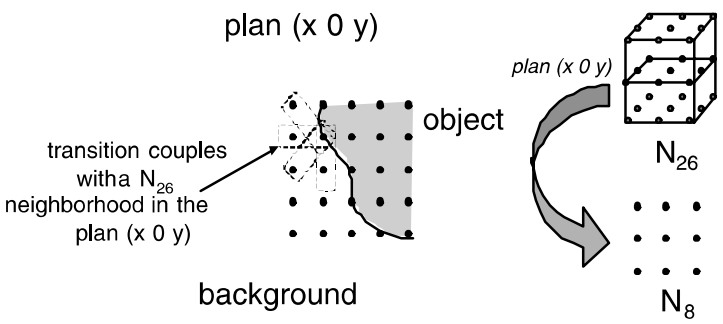
\includegraphics[width=0.6\textwidth]{figures/过渡对.png}
    \caption{过渡对}
    \label{fig:过渡对}
\end{figure}

Kohler(1981)\cite{kohler1981segmentation}提出了一种基于以下启发式的自动阈值方法:对比度越高的边界,越有可能对应于图像中真正的不连续(注意,这种启发式的方法在强对比的纹理图像背景下并不适用)。因此,最佳阈值取决于与该阈值相关的边界中最强的对比度。在我们的应用中,我们概括了Kohler的方法,并提出了 $f_{a}(\sigma_{max})$ 的三个定义,以评估分割后区域边界的质量。

$w_1(\sigma_{max})$ 基于对数图像处理(LIP)对比。Jourlin和Pinoli(1989)\cite{jourlin1989contrast}引入了一个新的数学模型,称为对数图像处理(LIP)模型,特别适合于对数图像,如X射线图像。在这种情况下,他们将两个像素之间的LIP对比度定义如下:

\begin{equation}
    \dots
\end{equation}
其中 $f$ 是灰阶函数,$M$ 是使得 $2^n$ 严格高于灰阶范围的最低值(例如,如果像素以8比特编码,$M=256$)。

我们定义 $w_1(\sigma_{max})$ 为 $B_{R(\sigma_{max})}$ 的所有过渡对(见\cref{fig:过渡对})的LIP对比之和,以过渡对总数 $N_{tc}$ 标准化:
\begin{equation}
    \dots
\end{equation}

$w_2(\sigma_{max})$ 基于标准差。对于 $B_{R(\sigma_{max})}$ 的每个像素 $x$ ,计算x和其不属于分割区域 $R(\sigma_{max})$ 的相邻像素(见\cref{fig:邻域})的标准差,表示为ξ(x)。设 $n$ 为邻居的数量。

我们将 $w_2(\sigma_{max})$ 定义为所有 $\xi (x)$ 的总和,被 $Card\{B_{R(\sigma_{max})}\}$(即:属于 $B_{R(\sigma_{max})}$ 的像素总数)标准化:

\begin{equation}
    \dots
\end{equation}

$w_3(\sigma_{max})$ 基于过渡水平。我们定义 $w_3(\sigma_{max})$ 为所有过渡对的过渡水平之和(见\cref{fig:过渡对}),被 $N_{tc}$ 标准化:
\begin{equation}
    \dots
\end{equation}

\subsection{基于区域的方法}

我们提出了三种基于区域标准的 $f_{a}(\sigma_{max})$ 的备选方案。

基于熵的 $S(\sigma_{max})$。一些作者(Pun, 1981\cite{pun1981entropic}; Kapur等人, 1985\cite{kapur1985new})将熵用于图像阈值处理。这种方法包括最大限度地提高所产生的图像熵,以最大限度地提高簇之间的对比度。

定义 $\overline{R}(\sigma_{max})$ 为 $R(\sigma_{max})$ 的补集区域。我们定义 $S(\sigma_{max})$ 为 $S_{R}(\sigma_{max})$ 和 $S_{\overline{R}}(\sigma_{max})$ 之和(见\hyperref[sec:appendix_a]{附录A}):
\begin{equation}
    \dots
\end{equation}

$V(\sigma_{max})$基于群组间的差异。Otsu(1979)\cite{otsu1979threshold}在因子判别分析的基础上实现了一种阈值技术,它包括寻找聚类之间的最佳分离。这个问题等同于最大化集群间的方差。

我们定义 $V(\sigma_{max})$ 为 $V_{R}(\sigma_{max})$ 和 $V_{\overline{R}}(\sigma_{max})$ 之和:
\begin{equation}
    \dots
\end{equation}

Inv$D_{GL}(\sigma_{max})$ 基于与灰阶函数的距离。Labouré(1987)\cite{laboure1987feasibility}提出通过用一个由平均簇构建的阶梯函数来接近灰阶函数来对图像进行阈值测定。阈值的确定包括检测灰度级函数和阶梯函数之间的最小距离。

设 $D_{GL}(\sigma_{max})$ 为原始图像的灰阶函数与平均值 $M_R$ 及 $M_{\overline{R}}$ 之间的距离:
\begin{equation}
    \dots
\end{equation}
当 $D_{GL}(\sigma_{max})$ 最小化时,得到的分割图像最适合原始图像。为了与之前的函数保持一致,将使用 $D_{GL}(\sigma_{max})$ 的倒数,即 Inv$D_{GL}(\sigma_{max})$。如果 $D_{GL}(\sigma_{max})$ 为空,Inv$D_{GL}(\sigma_{max})$ 将被放到最大的数值。

对于 $f_{a}(\sigma_{max})$ 的上述每一个表达式, $\sigma_{opt}$ 将通过检测使该函数最大化的值来确定。

\subsection{在人工图像上测试}\label{sec:test}

我们用一张测试图像来研究所提出的评估函数的行为。该图像由浅色背景(灰度=70)和其中的深色网格(灰度=25)组成(见\cref{fig:人工图像测试}(a)),并添加了平均值为0、标准差为10的高斯噪声(见\cref{fig:人工图像测试}(b))。这些属性被选作为我们的应用的代表。为了简单起见,这项研究是在二维进行的,因为维度并不改变评估函数的行为。因此,结果在三维中是可移植的。为了衡量分割的准确性,我们定义了一个系数
\begin{equation}
    \dots
\end{equation}
其中 $n_{common}$ 是分割后的网格和原始网格之间的共同像素数,$n_{grid}$ 是原始网格的像素数,$n_{segmented grid}$ 是分割后的网格的像素数。

\cref{fig:评估函数} 比较了归一化评估函数与 $\alpha$ 的关系。$\sigma = \sigma_{\alpha}$ 时,$\alpha$ 达到最大。由于 $\omega1,\omega2,\omega3$ 有相同的行为,为了更加清楚,我们只展示 $\omega3$。由于 $\omega1,\omega2,\omega3,V$ 和 Inv$D_{GL}$ 在接近 $\sigma_{\alpha}$ 的数值时达到最大,它们可以被用作 $f_{a}(\sigma_{max})$。$S$ 在 $\sigma \neq \sigma_{\alpha}$ 的值时达到最大,因此它不能被认可为这种类型的图像的可接受的评估函数。在\cref{fig:人工图像测试}(c)中,$\sigma_{\alpha} = 9.9$ 时获得了最佳分割。在\cref{fig:人工图像测试}(d)中,$\omega1,\omega2,\omega3$ 在 $\sigma_{opt} = 9.6$ 的情况下得到了相当的分割结果。在\cref{fig:人工图像测试}(e)中,$V$ 和Inv$D_{GL}$ 在$\sigma_{opt} = 10.2$ 的情况下给出了相似的结果。在\cref{fig:人工图像测试}(f)中,$S$ 未能找到最佳分割,其$\sigma_{opt} = 18.75$。

我们可以注意到,在\cref{fig:评估函数}中,$\omega3$ 在 $\sigma_{max}$ 的低值和高值的每个极端都在增加。这是由于存在孤立的、具有非常高的过渡边界的点所造成的。为了避免这些扰动,$\sigma_{max}$ 的变化被限制在第\cref{sec:arg_description}所述的范围内。在我们的应用中,这些不重要的部分通过选择 $\beta=0.5$ 而被抑制。 此外,由于图像具有双模直方图,意味着只有一个最大值的存在,因此有可能保持 $\sigma_{max}$ 的大范围变化。在多模态直方图的情况下,评价函数可能出现局部最大值。应调整 $\beta$ 的值以限制 $\sigma_{max}$ 的变化。

\begin{figure}[htbp]
    \centering
    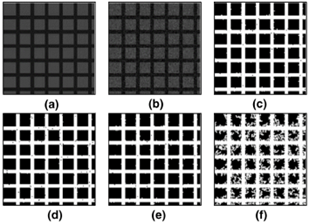
\includegraphics[width=0.5\textwidth]{figures/人工图像测试.png}
    \caption{(a) 原始图像; (b) 带高斯噪声的原始图像; (c) 当α=αmax的最佳分割区域;最佳区域: (d) 依据w1, w2, w3; (e) 依据V 和 InvDGL; (f) 依据 S.}
    \label{fig:人工图像测试}
\end{figure}

\begin{figure}[htbp]
    \centering
    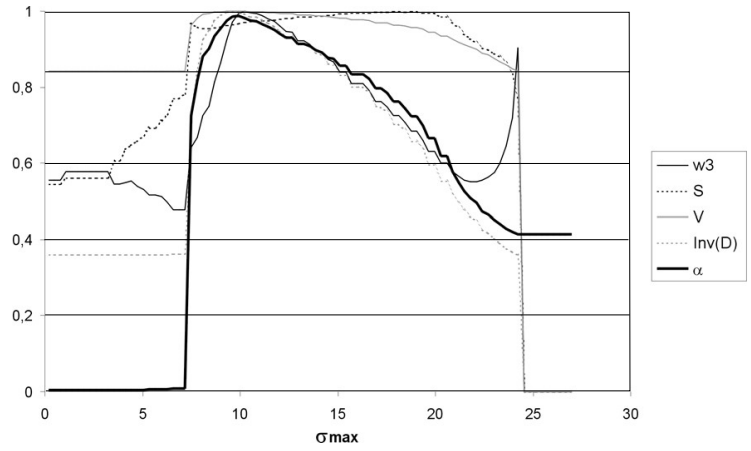
\includegraphics[width=0.5\textwidth]{figures/评估函数.png}
    \caption{系数α和由w1,w2,w3,S,V,InvDGL计算的归一化评估函数与σmax的关系}
    \label{fig:评估函数}
\end{figure}
